\subsection{Experimentación}

En la siguiente aparatado intentaremos validar dos hipótesis: que el modelo generado realmente puede ser identificado como un hablante extranjero y al mismo tiempo que este posee un grado de inteligibilidad aceptable.

Para eso se condujo una encuesta perceptual donde, dado un participante, se le presentó un audio con una oración semánticamente impredecible, fonéticamente balanceada y con distintos grados de mezcla de español e ingles, se le pidió que la transcribiera y que intentara identificar la nacionalidad del mismo.

Para la experimentación, se generaron diez oraciones distintas variando el nivel de mezcla de los modelos generados entre $30\%$ de ingles - $70\%$ castellano hasta $70\%$ de ingles - $30\%$ de castellano.

La encuesta se realizó a través de internet, con el mismo set de instrucciones para todos los participantes y pidiendo como requerimiento la utilización de auriculares. Cada participante podía contestar como máximo 5 veces a la encuesta (otorgandoseles audios siempre distintos).

La misma se llevó a cavo desde el 18 de octubre de 2017 hasta el primero de diciembre.

\subsubsection{Interface}

A continuación se presentará la interface que utilizamos para realizar la encuesta junto con las deciciones de diseño que fueron tomadas a lo largo de la misma. 

Todos los participantes al entrar en la pagina donde se hosteaba la encuesta se encontraron con lo siguiente:

Con el objetivo de no influir el las respuestas de los participantes participantes, procuramos no darles a los participantes en ningun momento información especifica de que buscabamos con este estudio.

A cada participante se le pidió como requerimiento que realizara la encuesta con auriculares y en un lugar silencioso.

Ademas, a cada participante le pedimos que indique su genero, su edad y la provincia en la que transcurrido la mayor parte de su infancia.

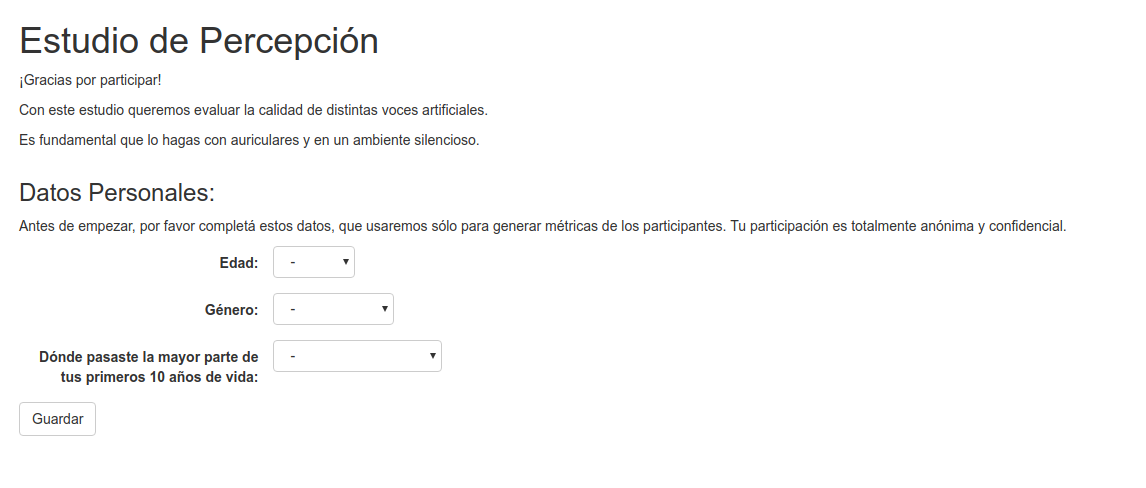
\includegraphics[scale=0.5]{estudio_online/estudio1.png}

Una vez que completaban esta información, y presionavan el boton de guardar, se les presentaba otra vista donde se le brindaban las instucciones necesarias para completar la encuesta:

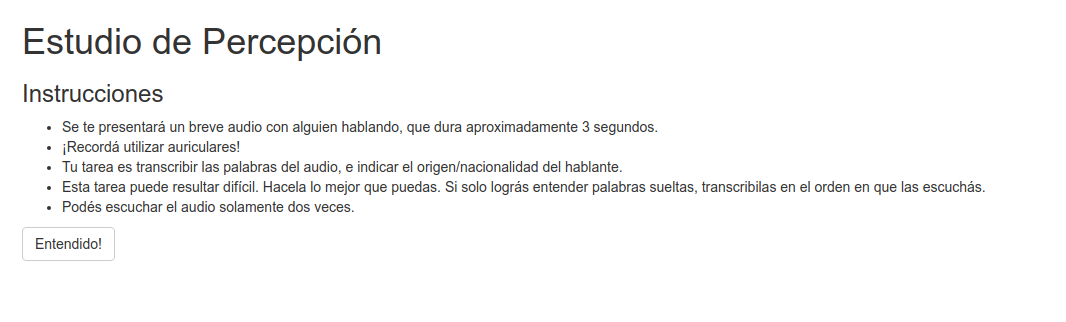
\includegraphics[scale=0.5]{estudio_online/estudio2.png}

Una vez que precionan el boton de "entendido!" les es presentado un audio, que pueden escuchar un maximo de 2 veces, una caja de texto libre donde escribir lo que interpretaron del mismo y una caja de texto libre donde escribir la nacionalidad que concideran es el hablante.

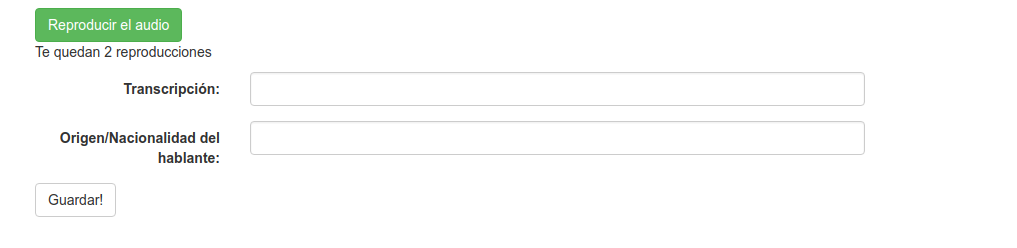
\includegraphics[scale=0.5]{estudio_online/estudio3.png}


Las oraciones presentadas fueron:

\begin{enumerate}
\item Mi montaña aguileña recorrió la esquina
\item Aquel fuerte vidrio prefirió aquel botón
\item Este enjoyado juez comprará nuestro corchete
\item Tu estrecho posavasos gritó la fechoría
\item Nuestro nublado tigre concluyó a este chupetin
\item Su profundo riñón apoyó a Julio
\item El frío churrasco oyó lo de polonia
\item Las acongojadas cotorras sonrieron a mi círculo
\item Ese gruñón perro prometió a esos cuñados
\item El nudillo Argentino perdió su vaso
\end{enumerate}


\subsection{Resultados}

Se encuestaron 109 participantes, con los que se obtuvieron 352 resultados.


A continuación presentaremos los datos demograficos de los participantes:

\begin{figure}[htp]
\begin{center}
$
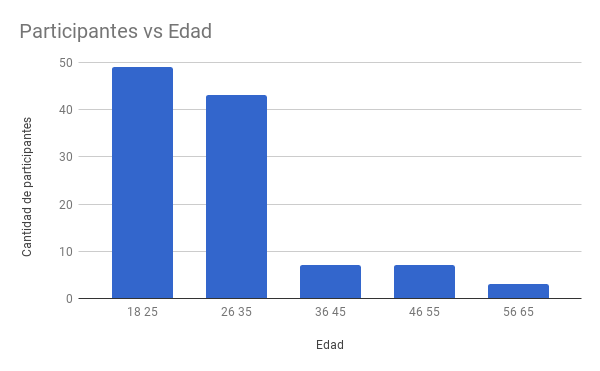
\includegraphics[scale=0.3]{datosDemograficos/edad.png}
$
\end{center}
\caption{Figure caption}
\label{pics:blablabla}
\end{figure}


En cuanto al genero de los participantes, 187 respuestas fueron brindadas por participantes del genero femenino mientras que 163 respuestas fueron respondidas por personas del genero masculino, una persona no contesto a esta pregunta.


\begin{figure}[htp]
\begin{center}
$
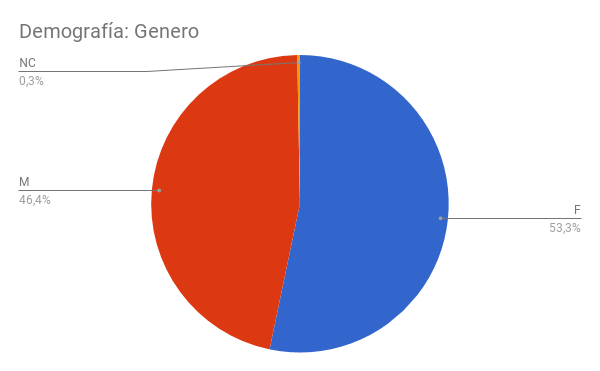
\includegraphics[scale=0.3]{datosDemograficos/genero.png}
$
\end{center}
\caption{Figure caption}
\label{pics:blablabla}
\end{figure}


Así mismo, la distribución de el lugar donde los participantes pasaron su infancia se puede ver en este grafico:


\begin{figure}[htp]
\begin{center}
$
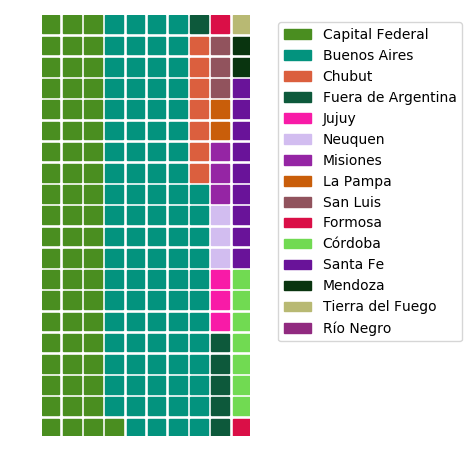
\includegraphics[scale=0.3]{datosDemograficos/infancia.png}
$
\end{center}
\caption{Figure caption}
\label{pics:blablabla}
\end{figure}

\subsubsection{Inteligibilidad}

Para el analisis de resultados utilizaremos la distancia de Levenshtein con inserciones, remociones y reemplazos. Respetando los acentos pero sin tener en cuenta mayusculas o minusculas.

Presentamos aquí los resultados obtenidos sin ningun tipo de modificación:

\begin{figure}[htp]
\begin{center}$
\begin{array}{lll}
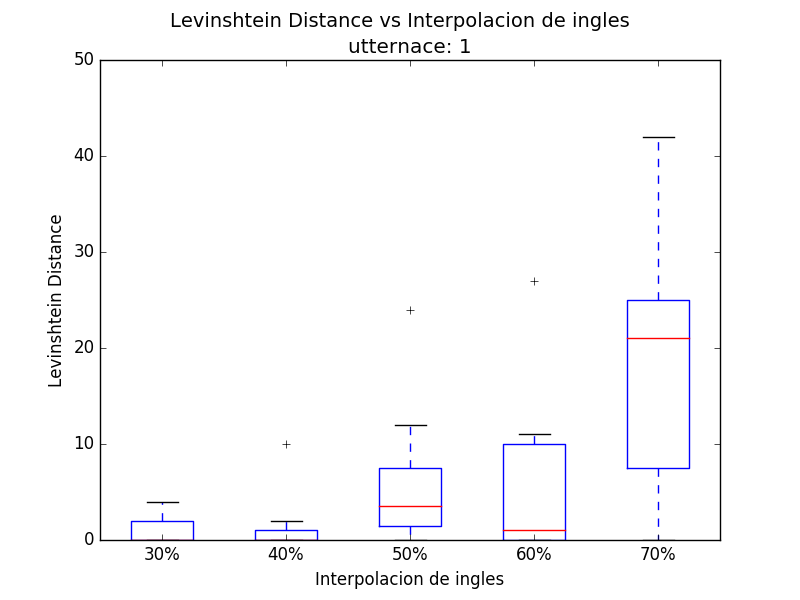
\includegraphics[width=.5\textwidth]{imagenes/plots_raw/1.png}&
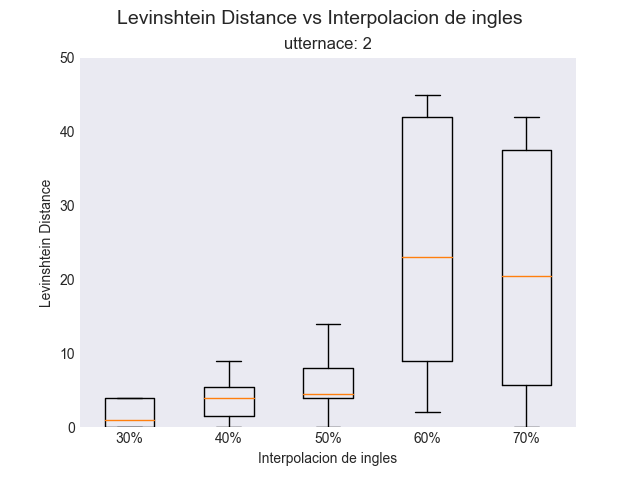
\includegraphics[width=.5\textwidth]{imagenes/plots_raw/2.png}
\end{array}$
\end{center}
\caption{Figure caption}
\label{pics:blablabla}
\end{figure}

\begin{figure}[htp]
\begin{center}$
\begin{array}{lll}
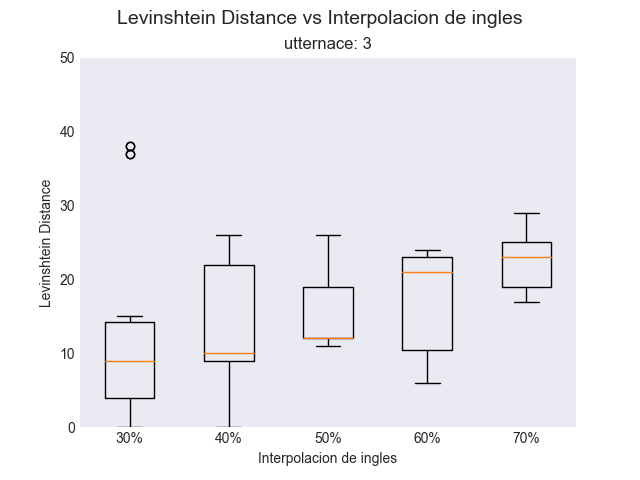
\includegraphics[width=.5\textwidth]{imagenes/plots_raw/3.png}&
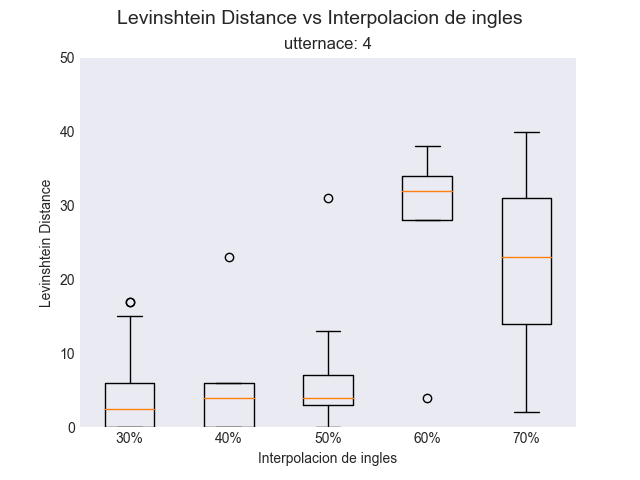
\includegraphics[width=.5\textwidth]{imagenes/plots_raw/4.png}
\end{array}$
\end{center}
\caption{Figure caption}
\label{pics:blablabla}
\end{figure}

\begin{figure}[htp]
\begin{center}$
\begin{array}{lll}
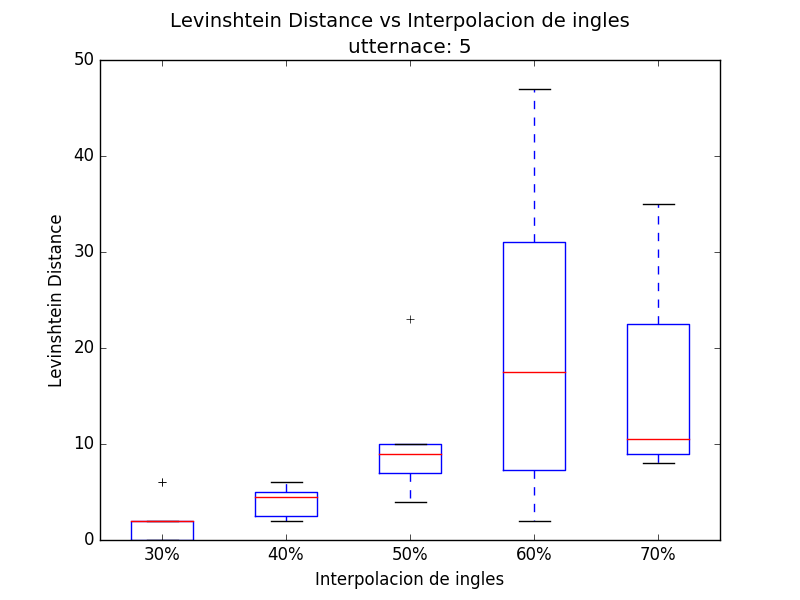
\includegraphics[width=.5\textwidth]{imagenes/plots_raw/5.png}&
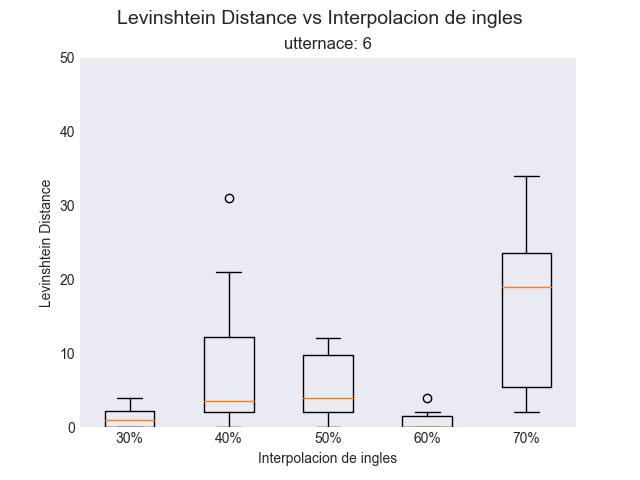
\includegraphics[width=.5\textwidth]{imagenes/plots_raw/6.png}
\end{array}$
\end{center}

\caption{Figure caption}
\label{pics:blablabla}
\end{figure}

\begin{figure}[htp]
\begin{center}$
\begin{array}{lll}
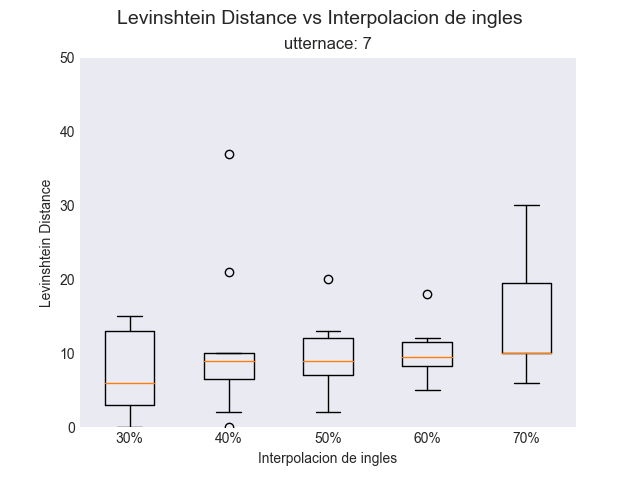
\includegraphics[width=.5\textwidth]{imagenes/plots_raw/7.png}&
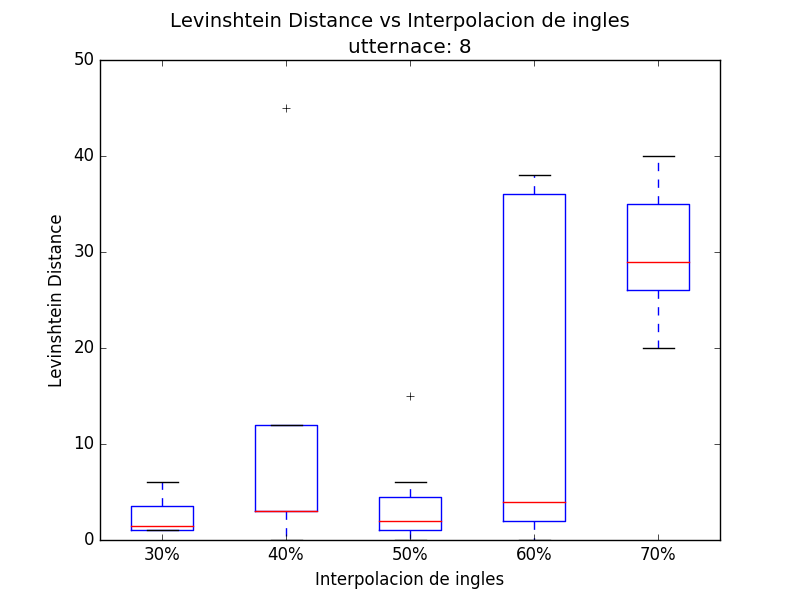
\includegraphics[width=.5\textwidth]{imagenes/plots_raw/8.png}
\end{array}$
\end{center}

\caption{Figure caption}
\label{pics:blablabla}
\end{figure}
\begin{figure}[htp]
\begin{center}$
\begin{array}{lll}
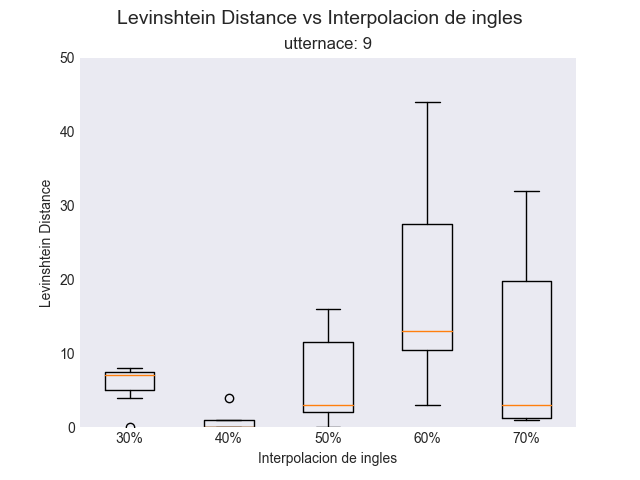
\includegraphics[width=.5\textwidth]{imagenes/plots_raw/9.png}\quad
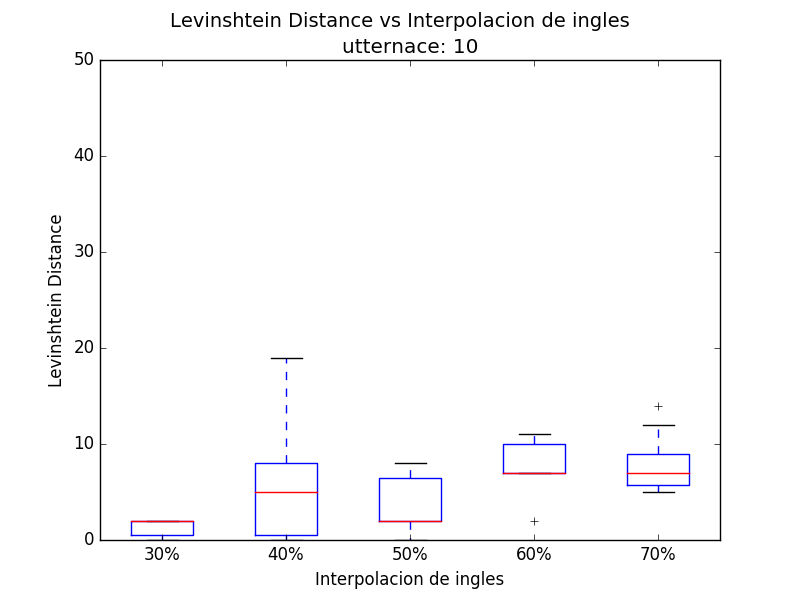
\includegraphics[width=.5\textwidth]{imagenes/plots_raw/10.png}
\end{array}$
\end{center}
\caption{Figure caption}
\label{pics:blablabla}
\end{figure}

Como puede verse en la mayoría de los utternaces se puede observar que hasta el $50\%$ de mezcla castellano-ingles, se conserva el un buen grado de inteligibilidad, rondando la distancia de Levenshtein al rededor de $10$ a $20$ caracteres. Pasados el $60\%$ de ingles, se observa una disminución bruzca en la inteligibilidad, llegando a una distancia de 45 caracteres.

Analizando mas detenidamente los datos obtenidos pudimos observar algunas fallas que podrían generar ruido en el analisis, tales como:

\begin{itemize}
	\item Los participantes escribieron de manera diferente cuando no entendieron un segmento del audio.
		\begin{itemize}
		\item Muchos de ellos escribieron: "...", "...." o simplemente omitían la palabra.
		\item En casos menos comunes: "***", "???", "blablabla".
		\end{itemize}
	\item En casos donde no comprendieron ninguna palabra del audio escribieron cosas como "no entendi nada", "nada", dejaron el campo vacío, etc.
	%\item Faltas ortografias del estilo: "grunion" en vez de "gruñón" que podría deberse a un teclado
	\item Utilización de signos de puntuación en las oraciones:
		\begin{itemize}
		\item Puntos finales para expresar el final de la oración o expresiones como "(?)".
		\item En un caso extremo, un participante el participante transcribió ""tu estrecho posavasos", grito la fechoría", cuando el utternace original solo decía "tu estrecho portavasos gritó la fechoría".
		\end{itemize}
	\item Omición de acentos en palabras que no resultaban ambiguas.
\end{itemize}

Para tener datos mas precisos, decidimos realizar una limpieza de los datos donde concideramos que no era disruptiva.

Los cambios fueron:

\begin{itemize}
\item corregir "ni" por "\~{n} " en la palabra grunion.
\item Remoción de todos los signos de puntuación. 
\item Remoción de expresiones como "blabla" o cualquier otra que exprese ininteligibilidad de una palabra u oración.
\item Correción de acentos en palabras no ambiguas: "botón", "prefirió", "recorrió", "chupetín", "riñón", "grúñón".
\item Las palabras que presentan ambibalencia, como : "concluyó" no fueron modificadas ya que concluyó/concluyo son validas.
%otros ejemplos: apoyo, enfrío
\end{itemize}

Habiendo realizado estas correcciones, ahora las distancias de Levinshtein se ven así: 

\begin{figure}[htp]
\begin{center}$
\begin{array}{lll}
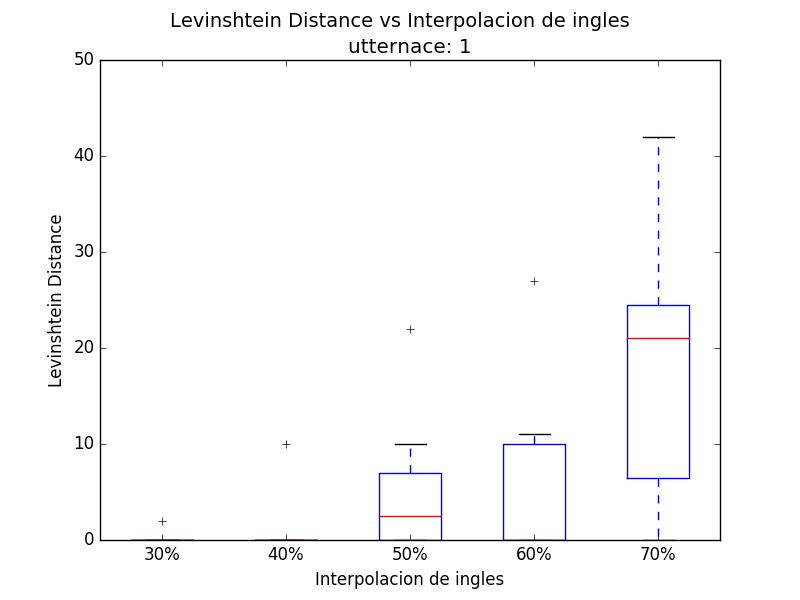
\includegraphics[width=.5\textwidth]{imagenes/plots_normalized/1.png}&
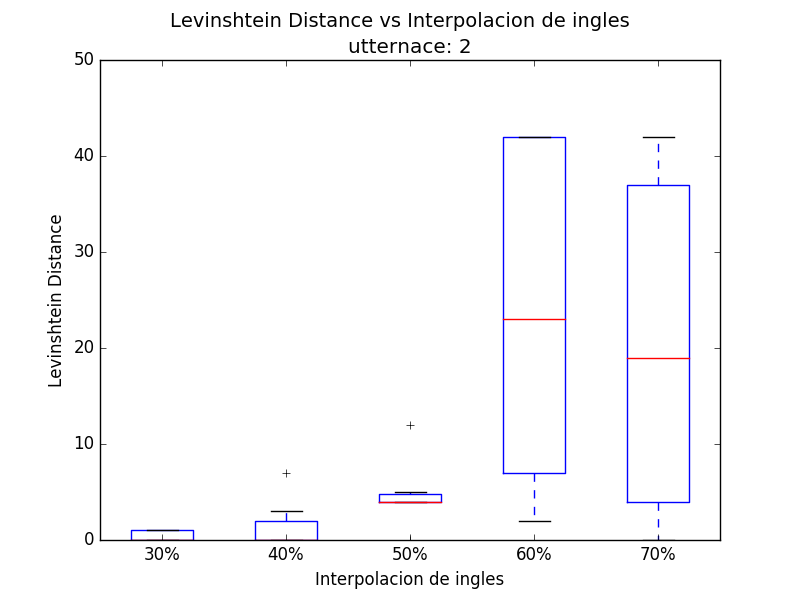
\includegraphics[width=.5\textwidth]{imagenes/plots_normalized/2.png}
\end{array}$
\end{center}
\caption{Figure caption}
\label{pics:blablabla}
\end{figure}

\begin{figure}[htp]
\begin{center}$
\begin{array}{lll}
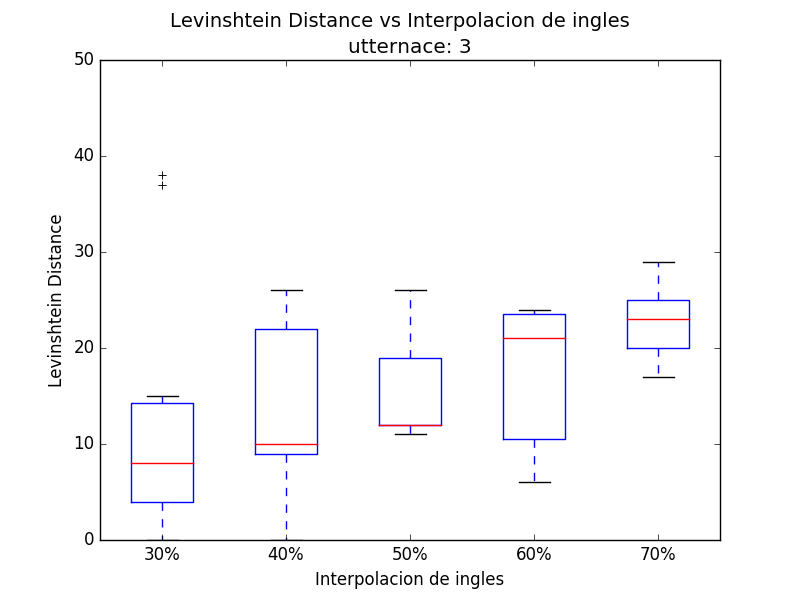
\includegraphics[width=.5\textwidth]{imagenes/plots_normalized/3.png}&
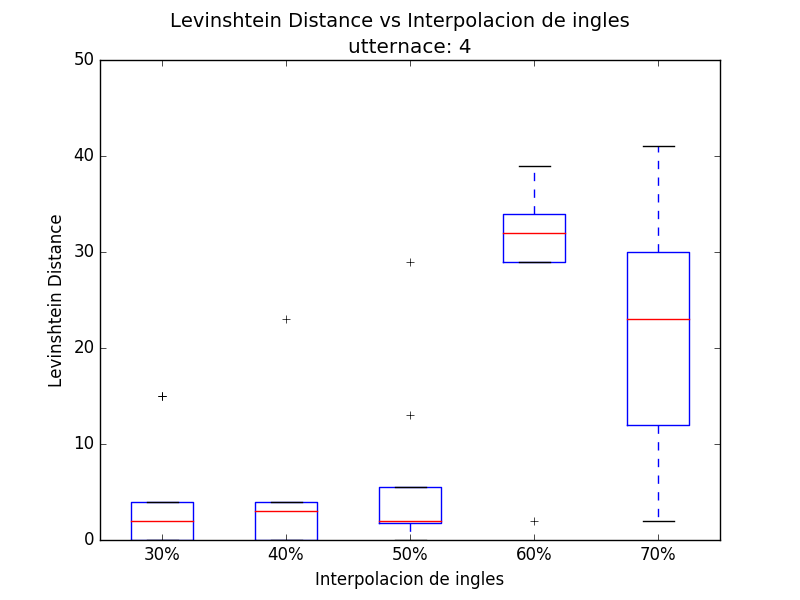
\includegraphics[width=.5\textwidth]{imagenes/plots_normalized/4.png}
\end{array}$
\end{center}
\caption{Figure caption}
\label{pics:blablabla}
\end{figure}

\begin{figure}[htp]
\begin{center}$
\begin{array}{lll}
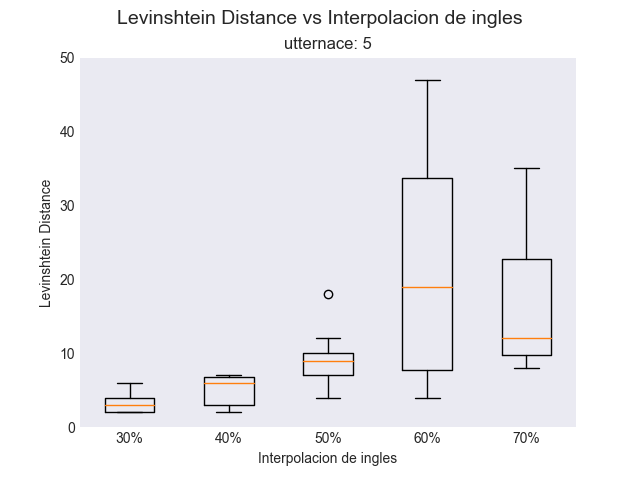
\includegraphics[width=.5\textwidth]{imagenes/plots_normalized/5.png}&
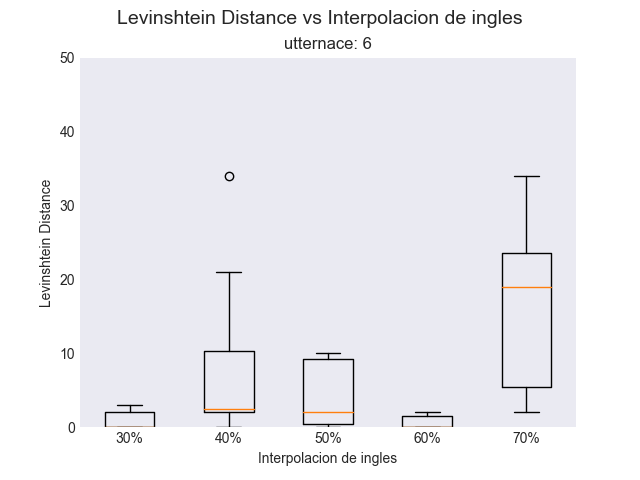
\includegraphics[width=.5\textwidth]{imagenes/plots_normalized/6.png}
\end{array}$
\end{center}

\caption{Figure caption}
\label{pics:blablabla}
\end{figure}

\begin{figure}[htp]
\begin{center}$
\begin{array}{lll}
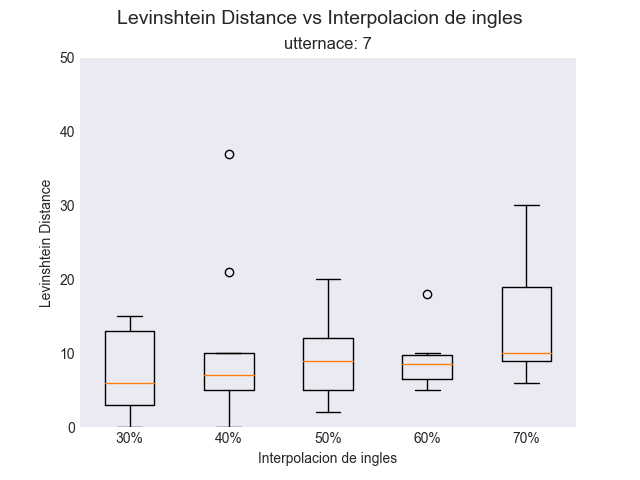
\includegraphics[width=.5\textwidth]{imagenes/plots_normalized/7.png}&
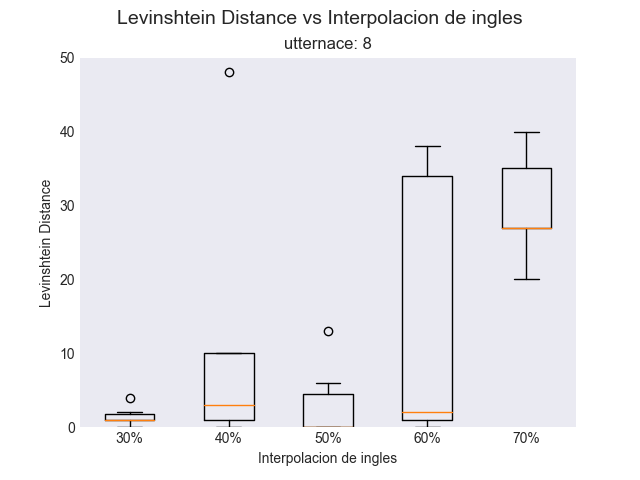
\includegraphics[width=.5\textwidth]{imagenes/plots_normalized/8.png}
\end{array}$
\end{center}

\caption{Figure caption}
\label{pics:blablabla}
\end{figure}
\begin{figure}[htp]
\begin{center}$
\begin{array}{lll}
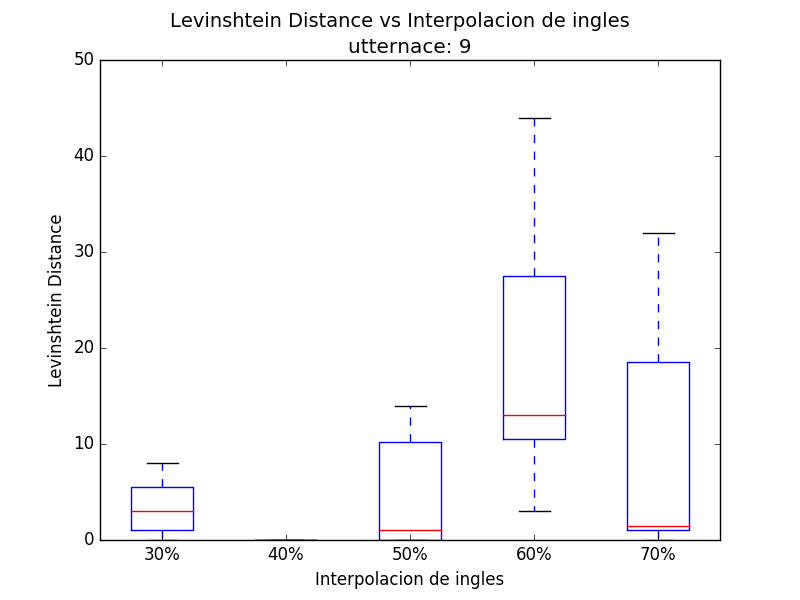
\includegraphics[width=.5\textwidth]{imagenes/plots_normalized/9.png}&
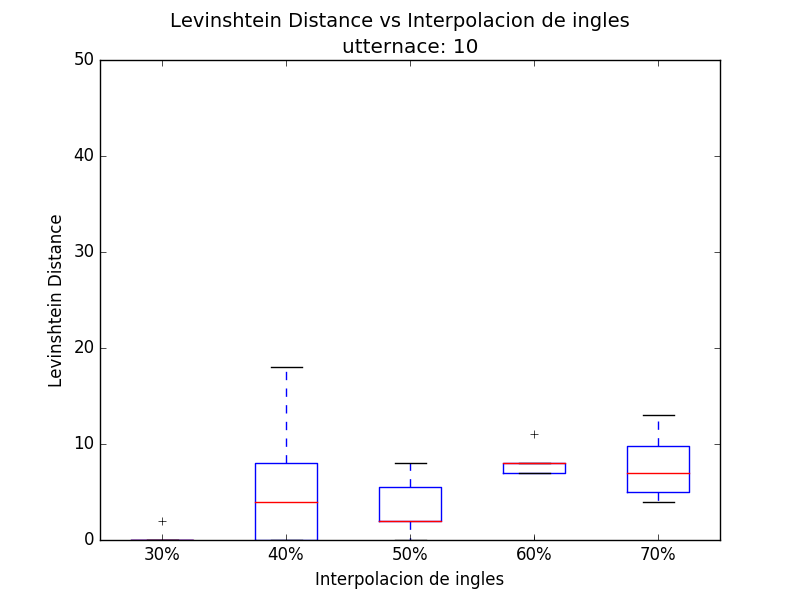
\includegraphics[width=.5\textwidth]{imagenes/plots_normalized/10.png}
\end{array}$
\end{center}
\caption{Figure caption}
\label{pics:blablabla}
\end{figure}

Con esta estandaricación de los datos, trataremos de darles un peso intuitivo que nos permitan sistematizar el analisis.

Por ejemplo, tomando una de las fraces utilizadas en la experimentación: 

\begin{itemize}
	\item "Las acongojadas cotorras sonrieron a mi círculo"
\end{itemize}

Podemos observar que:

\begin{itemize}
	\item Distancia 0: "Las acongojadas cotorras sonrieron a mi círculo"
	\item Distancia 10: "Las acontojadas culturas sonrieron en semicírculo"
	\item Distancia 20: "Plaza sombreada con sombrero sonrieron en mi círculo"
	\item Distancia 30: "sonrieron en mi círculo"
	\item Distancia 40: "círculo"
	\item Distancia 48: ""
\end{itemize}

A partir de esto, para este trabajo vamos a tomar que una distancia de Levinshtein

\begin{itemize}
	\item Distancia 0-10: Buena Inteligibilidad
	\item Distancia 10-20: Mediana Inteligibilidad
	\item Distancia 20-40: Baja Inteligibilidad
	\item Distancia 40-: Inteligibilidad nula
\end{itemize}

Con este baseline, podemos decir que en el rango de $30\%$ a $50\%$ todos los utternaces menos el 3 presentan un buen grado de inteligibilidad.

Dentro de este rango, los errores mas comunes varían desde falta de acentos en palabras como "concluyó" ambiguas hasta faltas de inteligibilidad en palabras con cierta complegidad como "aguileña" o "gruñon".

Para el utternace 3: "este enjoyado juez comprará nuestro corchete" observamos que la mayoría de los participantes cometieron errores al transcribir la palabra "juez" que confundieron de manera sistematica con palabras sonoramente similares como "fue", y "enjoyado" que transcribieron como "enfollado", "enrollado" y la conjugación exacta del verbo comprar.

Pasado el $50\%$ de mezcla de ingles, se puede observar una caida drastica en la inteligibilidad, mayormente en el utternace $2, 4, 5, 6, 8$y $9$. Tambien vemos que la variablidad aumenta drasticamente, por ejemplo, en el utternace $4$ con $60\%$ un participante fue capaz de transcribir con distancia $2$ el audio. Así mismo con $70\%$ dos participantes fueron capaces de transcribir el audio con una distancia menor $10$.


\subsection{Analisis de Nacionalidad}

En lo de elegir una nacionalidad:
Sinonimos: EEUU-EstadosUnidos, España-España (sur)
Cosas no muy especificas: "anglo", "Inglés/Estado Unidense", "Hablante nativo de inglés"
Cosas raras: "Brasiltiño", ".?", "robolandia"